\documentclass[10pt,a4paper]{article}
\usepackage[margin=2cm]{geometry}
\usepackage{amsmath,amssymb,booktabs,graphicx,caption,subcaption,xcolor,float,hyperref,tikz}
\usetikzlibrary{arrows.meta,positioning,calc}
\hypersetup{colorlinks=true,linkcolor=blue!50!black,urlcolor=blue!50!black}
\captionsetup{font=small,labelfont=bf}
\newcounter{diagram}
\newcommand{\diagramcaption}[1]{\refstepcounter{diagram}\par\smallskip\noindent{\small\textbf{Diagram~\thediagram.} #1}}
\title{\vspace{-1.2cm}\textbf{Tipping an undecided swarm}\\[2pt]
\large Simulation 1 (days and nights), setup \texttt{task003-nosolution}}
\author{LLM-free simulator; report of 14 October 2026; runs of 7 October 2026\\
\small Mirrors the Simulation 2 report on \texttt{task003-nosolution} of the same date, section by section.}
\date{}
\begin{document}
\maketitle
\vspace{-1cm}

\paragraph{How the simulator works.} The world, \texttt{task\_003}, has three candidate
allocations; A0 is the correct one. Each of 24 agents is given one true fact about it and reasons as
an exact Bayesian: its \emph{belief} is the exact probability of A0, A1 and A2 given the facts it
currently remembers. An episode has 30 rounds, each a day and a night. During the day the agents act
one at a time in a new random order: an agent reads $q$ posts drawn at random from a shared
\emph{board} (never its own), adds their facts to its memory, recomputes its belief, \emph{votes}
(\emph{argmax}: the most probable allocation; \emph{probability matching}: a vote drawn from its
belief) and posts one remembered fact that supports its vote, or nothing if none does. At night a
\emph{controller} with a target, A0 (truth) or A2 (false), reads $q_c$ agent posts; unless at least
75\% of them come from agents voting for its target, or what it read already proves its target, it
posts the $b$ facts from its own pool that best support its target. The board is then cleared,
keeping only the controller's new posts. At each dawn every remembered fact is forgotten with
probability $1-\rho$ and comes back if read again. Every episode is run three times with the same
random draws: without a controller, with the truth controller and with the false controller.

\paragraph{Summary.} 24 agents hold evidence that, pooled, is exactly a coin flip between
allocation A0 (the truth) and A2, with no proof available to anyone. A controller steers
toward A0 or A2 using one shared pool of facts. With agents that vote by
\textbf{probability matching} (the main case, as in Simulation 2), the swarm stays undecided on its
own, and \textbf{either controller tips it within a few days}; the truth controller's gain is
larger, mostly because the silent swarm already leans to A2. \textbf{A larger posting budget can
backfire}, because the pool has few facts per target. The controller \textbf{senses the swarm
accurately}. Measured by whether the swarm's \emph{collective decision} is the target, \textbf{the
cheapest controller already reaches the full gain} (about 10 facts posted over 30 nights), and large
budgets spend up to 18 times more for the same or a worse result. With \emph{argmax} voting the
silent swarm instead locks into unanimity and drifts to A2; that special case is in
Section~\ref{sec:drift}.

\section{Setup}

\begin{center}
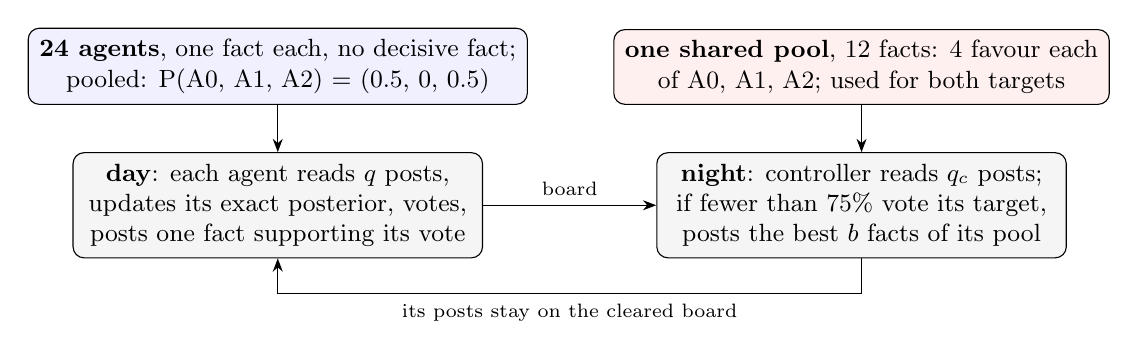
\begin{tikzpicture}[font=\small, box/.style={draw, rounded corners, align=center, inner sep=4pt}]
  \node[box, fill=gray!8, minimum width=5.2cm] (day) {\textbf{day}: each agent reads $q$ posts,\\
     updates its exact posterior, votes,\\ posts one fact supporting its vote};
  \node[box, fill=gray!8, right=2.2cm of day, minimum width=5.2cm] (night) {\textbf{night}: controller reads $q_c$ posts;\\
     if fewer than 75\% vote its target,\\ posts the best $b$ facts of its pool};
  \node[box, fill=blue!6, above=0.6cm of day, minimum width=5.2cm] (agents) {\textbf{24 agents}, one fact each, no decisive fact;\\
     pooled: P(A0, A1, A2) = (0.5, 0, 0.5)};
  \node[box, fill=red!6, above=0.6cm of night, minimum width=5.2cm] (pool) {\textbf{one shared pool}, 12 facts: 4 favour each\\
     of A0, A1, A2; used for both targets};
  \draw[-{Stealth}] (agents) -- (day);
  \draw[-{Stealth}] (pool) -- (night);
  \draw[-{Stealth}] (day) -- node[above, font=\scriptsize]{board} (night);
  \draw[-{Stealth}] (night.south) -- ++(0,-0.45) -| node[below, pos=0.25, font=\scriptsize]{its posts stay on the cleared board} (day.south);
\end{tikzpicture}
\diagramcaption{One round of Simulation 1, repeated for 30 rounds. Each dawn, every
remembered fact survives with probability $\rho$.}
\label{dia:setup}
\end{center}

No proof is available to anyone, not even if the controller posted its whole pool: the
agents' facts plus the whole pool give (0.75, 0, 0.25). The truth keeps an edge that
cannot be designed away (every fact is true): pooled agents plus the best part of the
pool reach at most P(A0) = 0.92, but P(A2) = 0.77.

Agents are exact Bayesian reasoners with posterior $P_j = (P_j(\text{A0}), P_j(\text{A1}), P_j(\text{A2}))$
over the facts they remember. They vote by one of two rules:
\begin{align}
\text{probability matching:}\quad & \Pr(\text{vote}_j = k) = P_j(k), \label{eq:pm}\\
\text{argmax:}\quad & \text{vote}_j = \arg\max_k P_j(k), \text{ ties broken at random.} \label{eq:argmax}
\end{align}
Control is measured by the \emph{paired gain}: each episode is run silent, with the truth
controller, and with the false controller, using the same random draws, and
\begin{equation}\label{eq:gain}
G_t^{(a)} = \frac{1}{E}\sum_{e=1}^{E}\Bigl[x_{a,t}^{\text{ctrl}}(e) - x_{a,t}^{\text{silent}}(e)\Bigr],
\end{equation}
where $x_{a,t}$ is the share of agents voting $a$ on day $t$, $E = 1000$ episodes. (Simulation 2
measures the gain in mean \emph{belief}; Figure~\ref{fig:votes} shows the vote shares of both
simulations on the same scale.) The grid: $q \in \{3,6,12\}$, $q_c \in \{3,6,12,24\}$,
$b \in \{1,2,3,6,9\}$, $\rho \in \{0.75, 1\}$. Unless stated otherwise: probability matching,
$q = 6$, $q_c = 12$, $b = 3$.

\section{Main result: both controllers tip the swarm within days}

\begin{figure}[H]
\centering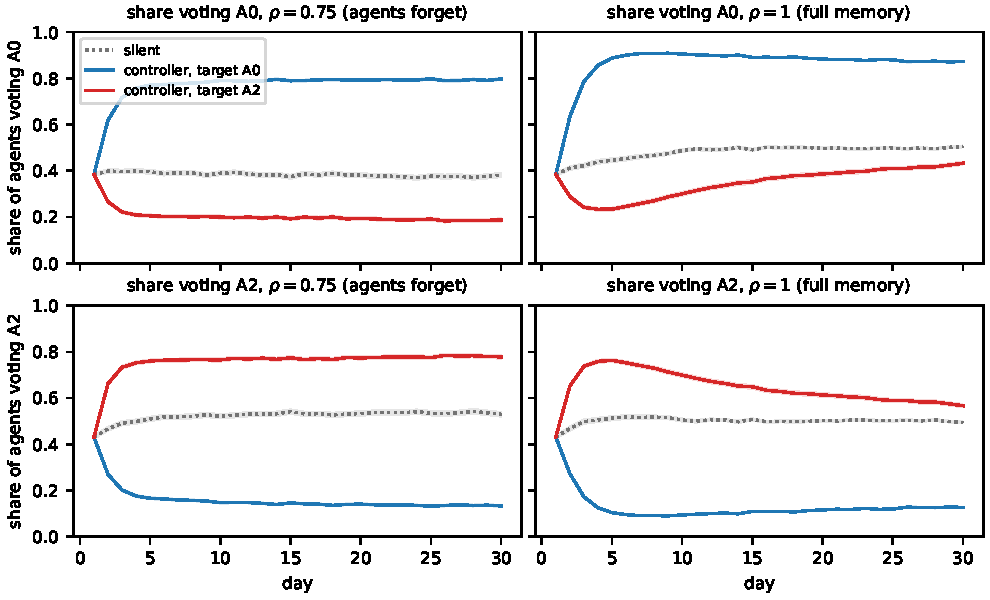
\includegraphics[width=0.84\linewidth]{figures/fig_votes_time.pdf}
\caption{Share of the 24 agents voting A0 (top) and A2 (bottom) at the end of each day, without a
controller (dotted grey), with the controller targeting A0 (blue) and with the one targeting A2 (red);
$\rho = 0.75$ (left) and $\rho = 1$ (right). Bands: 95\% intervals. Probability matching, $q = 6$,
$q_c = 12$, $b = 3$.}
\label{fig:votes}
\end{figure}

\begin{itemize}\itemsep1pt
\item \textbf{Without a controller the swarm stays split}: on day 30, 38\% vote A0 and 53\% A2 when
  agents forget, 50\% each with full memory. No episode becomes unanimous. The lean to A2 when agents
  forget comes from A2-side facts surviving forgetting better (held by 53\% of agents on day 30,
  A0-side facts by 31\%).
\item \textbf{Either controller tips it within about three days}: the target's share reaches 0.80
  (A0) or 0.78 (A2) when agents forget, and 0.87 (A0) or 0.57 (A2) with full memory.
\item \textbf{With full memory the false controller's lead erodes}: the A2 share peaks at 0.76
  (day 5) and falls to 0.57 by day 30, as agents accumulate the evidence that favours A0.
\end{itemize}

\begin{table}[H]
\centering\small
\caption{Probability matching, day 30, $q_c = 12$, $b = 3$: paired gain in the target's
share, Eq.~(\ref{eq:gain}), for $q = 3 / 6 / 12$; and the share of episodes in which
the target passes 75\% by day 30 (mean over $q$), with the silent value in brackets.}
\label{tab:pm}
\begin{tabular}{llccc}
\toprule
$\rho$ & controller & gain ($q = 3 / 6 / 12$) & target past 75\% & median day \\
\midrule
0.75 & truth (A0) & 0.33 / 0.42 / 0.43 & 0.99 (0.26) & 3--4 \\
0.75 & false (A2) & 0.21 / 0.25 / 0.23 & 0.98 (0.58) & 3 \\
1.0 & truth (A0) & 0.37 / 0.37 / 0.38 & 1.00 (0.36) & 3 \\
1.0 & false (A2) & 0.08 / 0.07 / 0.06 & 0.90 (0.47) & 3 \\
\bottomrule
\end{tabular}
\end{table}

\begin{figure}[H]
\centering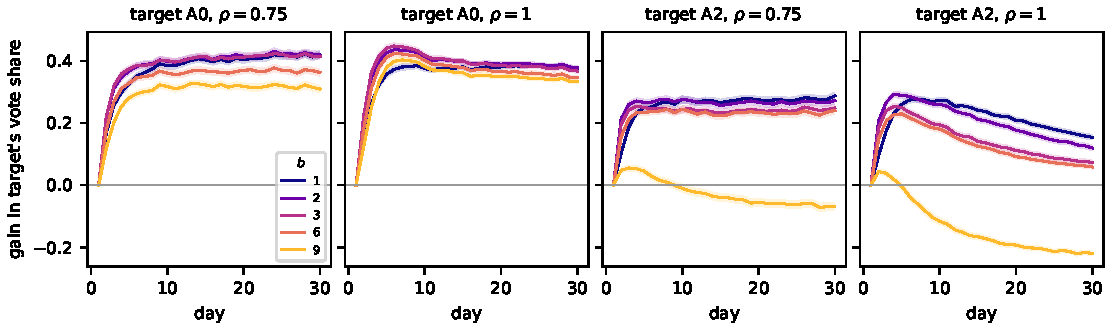
\includegraphics[width=0.98\linewidth]{figures/fig_gain_time.pdf}
\caption{Paired gain in the target's vote share over the days, Eq.~(\ref{eq:gain}), one line per
posting budget $b$. Bands: 95\% intervals.}
\label{fig:gaintime}
\end{figure}

\begin{figure}[H]
\centering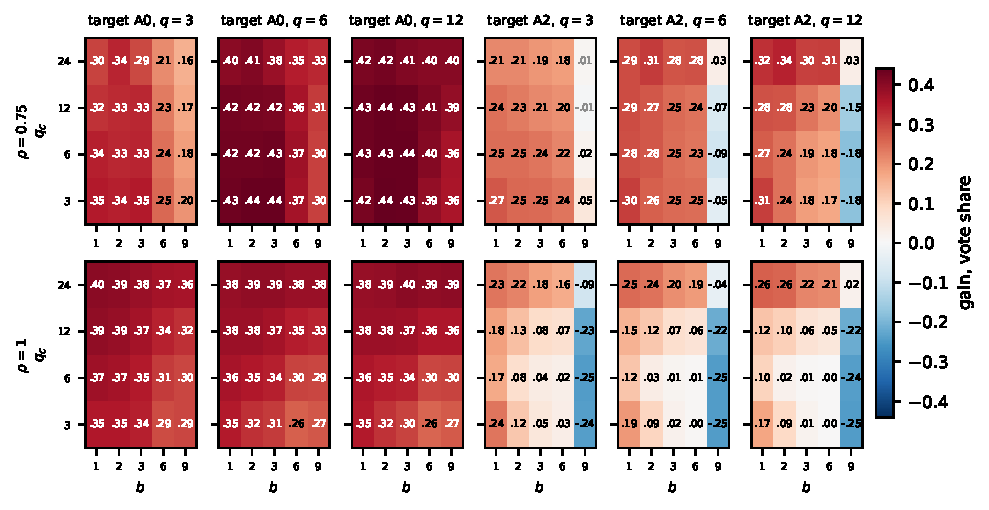
\includegraphics[width=0.98\linewidth]{figures/fig_phase_gain.pdf}
\caption{Day-30 paired gain over the facts per night $b$ (x) and the posts the controller reads
$q_c$ (y), for each target and every $q$ (columns), $\rho = 0.75$ and $1$ (rows). Grey number: the
95\% interval includes 0.}
\label{fig:phase}
\end{figure}

\begin{itemize}\itemsep1pt
\item \textbf{Both controllers tip the swarm in about 3 days} (Table~\ref{tab:pm}).
\item \textbf{The truth controller's gain is larger}, and the gap widens with full memory:
  about 0.37 against 0.07 at $\rho = 1$. When agents forget, the silent swarm already leans to A2,
  so there is more room to raise A0. With full memory, agents accumulate facts and their pooled
  evidence pulls back toward the truth's higher ceiling; the false controller's gain decays over
  the days (Figure~\ref{fig:gaintime}, right).
\item \textbf{The reading budget $q_c$ matters little}; the posting budget matters at its
  largest values (Section~\ref{sec:strength}).
\end{itemize}

\section{The controller's strength and the vote gate}\label{sec:strength}

\subsection{Strength: the posting budget}

\begin{figure}[H]
\centering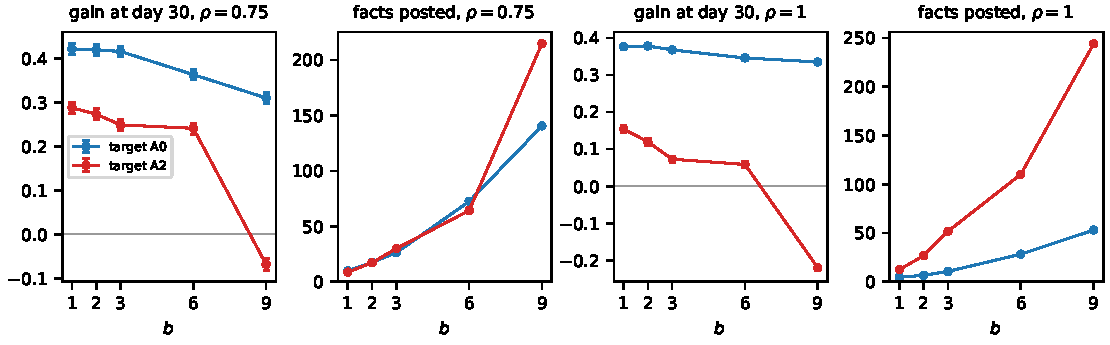
\includegraphics[width=0.98\linewidth]{figures/fig_strength.pdf}
\caption{Day-30 gain and facts posted (mean per episode, over 30 nights) against the facts per night
$b$, for $\rho = 0.75$ and $\rho = 1$ (target A0 blue, A2 red); $q = 6$, $q_c = 12$. Bars: 95\% intervals.}
\label{fig:strength}
\end{figure}

\paragraph{More budget can be worse: a design effect.} The gain falls as $b$ grows, and the
false controller's turns negative at $b = 9$ ($-0.07$ at $\rho = 0.75$, $-0.22$ at $\rho = 1$),
while the facts posted rise from about 10 to 140--245 per episode (Figure~\ref{fig:strength}). The
cause is arithmetic, not swarm dynamics. The controller must post exactly $b$ facts or none, and the
shared pool holds only $n_{\text{target}}$ facts on its target's side, so each post contains at least
\begin{equation}\label{eq:counter}
c = \max(0,\; b - n_{\text{target}})
\end{equation}
facts that do not favour its target.

\begin{table}[H]
\centering\small
\caption{Pool composition and what the false controller actually posts (probability
matching, $\rho = 1$, $q = 6$, $q_c = 12$). Tied facts count for both sides.}
\label{tab:budget}
\begin{tabular}{lccc}
\toprule
 & $b = 3$ & $b = 6$ & $b = 9$ \\
\midrule
facts in the pool on the target's side ($n_{\text{target}}$) & \multicolumn{3}{c}{A0: 4, \; A2: 6} \\
posted facts favouring A0 / A1 / A2 & 14 / 23 / 62\% & 12 / 22 / 67\% & \textbf{26} / 23 / 51\% \\
nights the controller posts & 59\% & 63\% & \textbf{93\%} \\
\bottomrule
\end{tabular}
\end{table}

The sharp fall starts exactly where Eq.~(\ref{eq:counter}) becomes positive: at $b = 6$ for the
truth controller ($n = 4$), at $b = 9$ for the false one ($n = 6$). Its counter-evidence
keeps the target's vote share below the gate, so it keeps posting (Table~\ref{tab:budget}),
and the counter-evidence accumulates. The effect replicates with fresh random draws
(a second seed). It disappears if the controller may post \emph{up to} $b$ facts, or never posts
facts against its target.

\paragraph{With full memory, more posts steer less even before that.} At $\rho = 1$ the false
controller's gain falls from $0.15$ at $b = 1$ to $0.06$ at $b = 6$, where Eq.~(\ref{eq:counter}) is
still zero. This is the same direction as the rate reversal of Simulation 2, where every additional
\emph{different} pool fact in circulation pulls beliefs toward the full-pool point (0.75, 0, 0.25)
whatever the target; whether the same mechanism acts here has not been tested.

\subsection{The vote gate}

Simulation 1 has no gate-off arm: the controller is always silent when at least 75\% of the posts it
reads come from agents voting for its target. With few posts read the gate is effectively stricter
($q_c = 3$: all 3 posts; $q_c = 6$: 5 of 6). Under probability matching the swarm stays mixed, so the
controller posts on most nights (59--93\%, Table~\ref{tab:budget}).

\section{The controller senses the swarm accurately}

Each night the controller estimates the share of agents backing its target from the
$n \le q_c$ agent posts it reads, $\hat v = \frac{1}{n}\sum_i \mathbb{1}\{\text{author of
post } i \text{ voted for the target}\}$, and stays silent when $\hat v \ge 0.75$.

\begin{figure}[H]
\centering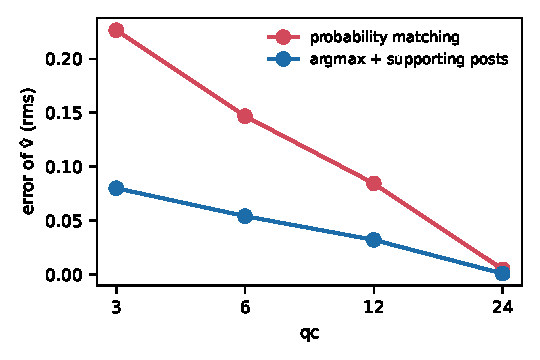
\includegraphics[width=0.45\linewidth]{figures/fig_sensing.pdf}
\caption{Error of $\hat v$ against the true share of all 24 agents, task003-nosolution.}
\label{fig:sensing}
\end{figure}

$\hat v$ is unbiased ($\pm 0.0005$), its error shrinks with $q_c$ and vanishes at
$q_c = 24$ (Figure~\ref{fig:sensing}). It is larger under probability matching because
those swarms stay mixed, which also makes gate mistakes more common: the controller
stays silent although the true share is below 0.75 on 5--8\% of nights, and posts
although it is above 0.75 on up to 13\% at $q_c = 3$. Abstaining agents (0.1--0.2\% of
agent-days) do not bias it. In Simulation 2, by contrast, $\hat v$ is biased upward.

%% ---------------------------------------------------------------------------------------------
\section{How readable is the command? Information and pair efficiency}\label{sec:eff}

A controller can change the swarm in two ways: in the direction it is asked to, or in ways that
happen whatever its target. We measure how readable the command is in the swarm (the mutual
information between the target and the swarm's state), which share of the change is directed (the
pair efficiency $\eta$), and how unsure the agents become. Throughout, the target is chosen by a fair
coin, and all quantities are taken at one time $t$, across the 1{,}000 episodes of each arm (not over
whole trajectories). Setting: probability matching, $q = 6$.

\subsection{Measures}

\begin{center}
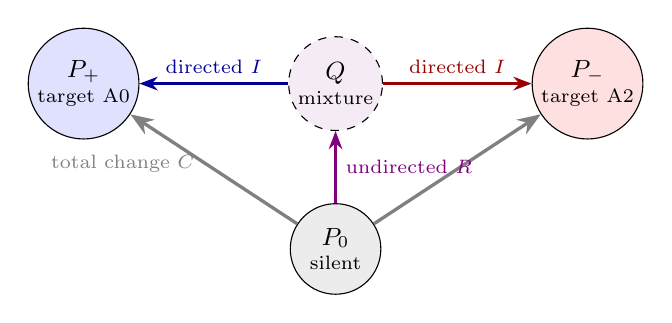
\begin{tikzpicture}[font=\small, dist/.style={draw, circle, minimum size=1.15cm, align=center, inner sep=1pt}]
  \node[dist, fill=gray!15] (P0) at (0,0) {$P_0$\\[-2pt]{\scriptsize silent}};
  \node[dist, fill=blue!12] (Pp) at (-3.2,2.1) {$P_+$\\[-2pt]{\scriptsize target A0}};
  \node[dist, fill=red!12] (Pm) at (3.2,2.1) {$P_-$\\[-2pt]{\scriptsize target A2}};
  \node[dist, dashed, fill=violet!8] (Q) at (0,2.1) {$Q$\\[-2pt]{\scriptsize mixture}};
  \draw[-{Stealth}, very thick, gray] (P0) -- node[left, font=\scriptsize, pos=0.55]{total change $C$} (Pp);
  \draw[-{Stealth}, very thick, gray] (P0) -- (Pm);
  \draw[-{Stealth}, thick, violet] (P0) -- node[right, font=\scriptsize]{undirected $R$} (Q);
  \draw[-{Stealth}, thick, blue!60!black] (Q) -- node[above, font=\scriptsize]{directed $I$} (Pp);
  \draw[-{Stealth}, thick, red!60!black] (Q) -- node[above, font=\scriptsize]{directed $I$} (Pm);
\end{tikzpicture}
\diagramcaption{Three distributions of the swarm's state at time $t$, one per arm, each over the
episodes of that arm. The controller's total change $C$ splits exactly into a part that depends on
its target ($I$, from the mixture $Q$ to each arm) and a part that does not ($R$, from silence to
$Q$). Efficiency $\eta = I/C$ is the directed share.}
\end{center}

\noindent\textbf{Distributions.} For each arm $a$ (silent $0$, target A0 $+$, target A2 $-$) and a
time $t$, each episode $e$ contributes a probability vector $y_a(e)$ over the values $x$ of the
state $X$: at \emph{one-agent} level its vote shares (the vote of a randomly chosen agent), at
\emph{swarm} level a mark on the bin of $s = m_{\text{A0}} - m_{\text{A2}}$ (difference of mean
beliefs, three equal bins on $[-1,1]$). Then $\hat P_a = \frac1n\sum_e y_a(e)$. Any pair of controllers
can be written as
\begin{equation}\label{eq:split}
\hat P_\pm = \hat P_0 + \mu \pm \delta,\qquad \mu = \tfrac12(\hat P_+ + \hat P_-) - \hat P_0,\quad
\delta = \tfrac12(\hat P_+ - \hat P_-),
\end{equation}
a \emph{common} part $\mu$ (what control does on average, whatever the target) and a
\emph{directional} part $\delta$; both are vectors over the values of $X$ (all answers, A1 included).

\noindent\textbf{Readability and the pair efficiency.} With $\hat Q = \hat P_0 + \mu$ and
$\mathrm{KL}(p\Vert q) = \sum_x p(x)\log_2[p(x)/q(x)]$,
\begin{equation}\label{eq:eta}
I = \tfrac12\mathrm{KL}(\hat P_+\Vert\hat Q) + \tfrac12\mathrm{KL}(\hat P_-\Vert\hat Q),\quad
C = \tfrac12\mathrm{KL}(\hat P_+\Vert\hat P_0) + \tfrac12\mathrm{KL}(\hat P_-\Vert\hat P_0) = I + R,\quad
R = \mathrm{KL}(\hat Q\Vert\hat P_0),\quad \eta = I/C .
\end{equation}
$I$ is the mutual information between the target and the state: how readable the command is
(at most 1 bit). With the one-agent state it is $I(\text{target};\text{vote of a randomly chosen
agent})$, the quantity mapped in Figure~\ref{fig:effI}. $I = \frac12\mathrm{KL}(\hat Q+\delta\Vert\hat Q) + \frac12\mathrm{KL}(\hat Q-\delta\Vert\hat Q)$
depends on $\delta$ and on where the pair sits ($\hat Q$); $R = \mathrm{KL}(\hat P_0+\mu\Vert\hat P_0)$ depends
only on $\mu$; $C$ (a number) $= I + R$, so $R = C - I$. The reference $\hat P_0$ is the silent arm. For
small changes, $\mathrm{KL}(p+\epsilon\Vert p) \approx \sum_x \epsilon(x)^2/(2\ln 2\,p(x))$ gives
\begin{equation}\label{eq:etasmall}
I \approx \frac{\Vert\delta\Vert^2}{2\ln 2},\quad R \approx \frac{\Vert\mu\Vert^2}{2\ln 2},\quad
\eta \approx \frac{1}{1 + \Vert \mu\Vert^2/\Vert\delta\Vert^2},\qquad \Vert v\Vert^2 = \sum_x \frac{v(x)^2}{\hat P_0(x)} .
\end{equation}
So $\eta = 1$ exactly when the two controllers' changes are mirror images ($\mu = 0$), whatever their
size, and $\eta$ falls only through the \emph{ratio} of common to directional change: when both push
the same way (a common push), or one moves the swarm much more than the other (a lopsided pair:
along one direction with sizes $a$ and $b$, $\Vert \mu\Vert/\Vert\delta\Vert = |a-b|/(a+b)$). It is a
property of the pair, not of either controller, and it stays constant whenever both effects grow
together; the size of the effect is measured by $I$. At swarm level $C$ is often infinite (the
controlled swarm reaches states silence never visits); there we use $\eta_{JS} = I/(I + \mathrm{JS}(\hat Q,\hat P_0))$ with the bounded
Jensen--Shannon divergence; $\mathrm{JS}(\hat Q,\hat P_0)$ is the information the state carries about
\emph{whether} a controller is present (controlled or silent, 50/50), so $\eta_{JS}$ compares
information about the direction with information about the presence of control.

\noindent\textbf{The agents' own uncertainty}: $\Delta\bar H$ (change in the mean entropy of their
beliefs) and $\Delta$JSD (change in disagreement, the entropy of the mean belief minus $\bar H$),
controlled minus silent, same episode.

\subsection{Over time}

\begin{figure}[!htb]
\centering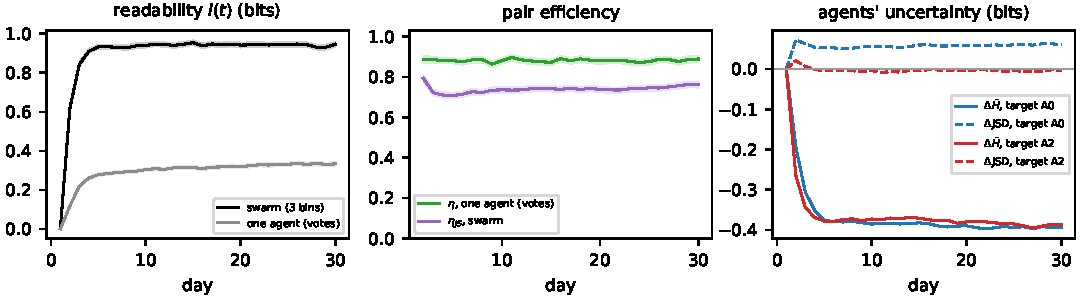
\includegraphics[width=0.92\linewidth]{figures/fig_eff_time2.pdf}
\caption{At $\rho = 0.75$, $q_c = 12$, $b = 3$ (end of each day): readability $I(t)$ at swarm and
one-agent level, pair efficiency ($\eta$, one agent; $\eta_{JS}$, swarm), and the change in the
agents' uncertainty. Bands: 95\% intervals over episodes.}
\label{fig:efftime2}
\end{figure}

\begin{figure}[!htb]
\centering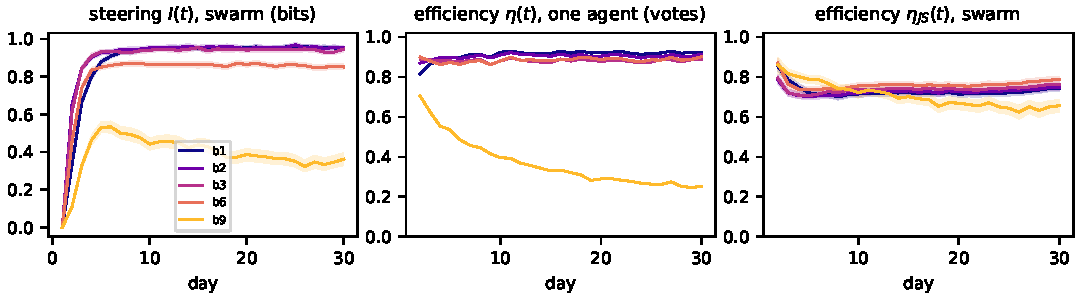
\includegraphics[width=0.66\linewidth]{figures/fig_eff_time.pdf}
\caption{Readability and pair efficiency over the days, $\rho = 0.75$, $q_c = 12$, one line per
facts per night $b$. Bands: 95\% intervals.}
\label{fig:efftime}
\end{figure}

\begin{itemize}\itemsep1pt
\item \textbf{Readability is reached within a few days and then stays}: $I = 0.84$ bits (swarm) on
  day 3 and $0.95$ on day 30; one agent's vote carries $0.22$ bits on day 3 and $0.33$ on day 30;
  $\eta = 0.89$, $\eta_{JS} = 0.76$.
\item \textbf{Both controllers make agents surer} ($\Delta\bar H \approx -0.39$ bits); the truth
  controller also splits them a little ($\Delta$JSD $+0.06$).
\end{itemize}

\subsection{Across the control plane}

\begin{figure}[!htb]
\centering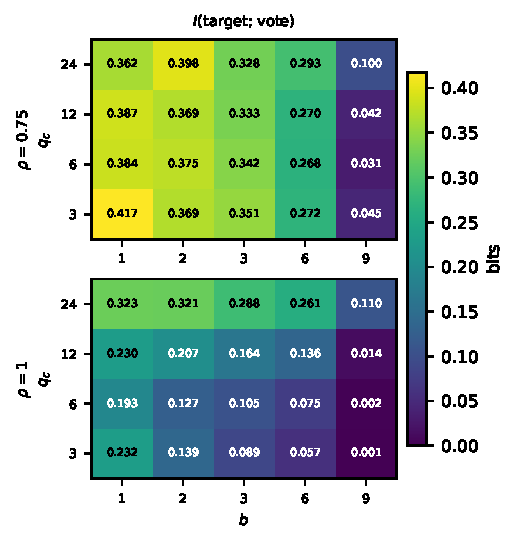
\includegraphics[width=0.36\linewidth]{figures/fig_eff_phase_I.pdf}
\caption{Readability $I(\text{target};\text{vote})$ at day 30, in bits, over the reading budget $q_c$ (y)
and the facts per night $b$ (x); state: the vote of a randomly chosen agent.}
\label{fig:effI}
\end{figure}

\begin{figure}[!htb]
\centering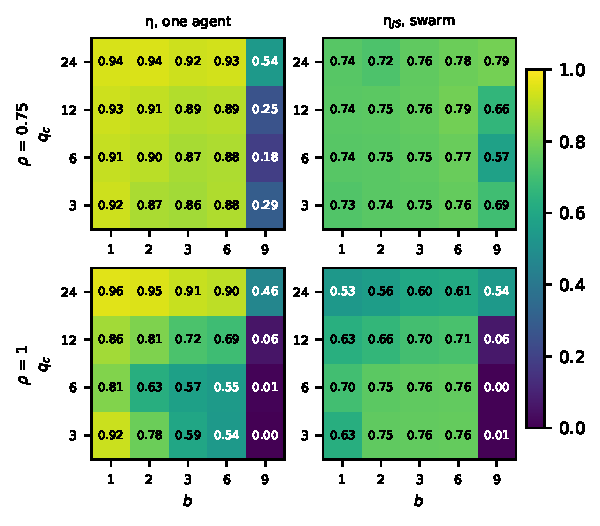
\includegraphics[width=0.36\linewidth]{figures/fig_eff_phase.pdf}
\caption{Pair efficiency at $t = 30$ over $q_c$ and the facts per night $b$: one-agent $\eta$ (beliefs) and swarm
$\eta_{JS}$. Dash: undefined.}
\label{fig:effphase}
\end{figure}

\begin{itemize}\itemsep1pt
\item \textbf{When agents forget, readability is high up to $b = 6$} (0.27--0.42 bits) and
  \textbf{collapses at $b = 9$} (0.03--0.10): the false controller's backfire makes its swarm look
  like the truth controller's.
\item \textbf{With full memory readability falls with $b$ and rises with $q_c$}: 0.19--0.32 bits at
  $b = 1$, 0.06--0.26 at $b = 6$, near 0 at $b = 9$ (up to 0.11 at $q_c = 24$), mirroring the false
  controller's falling gain (Figure~\ref{fig:phase}, bottom row).
\end{itemize}

\subsection{Readability, pair efficiency and uncertainty against the facts per night}

\begin{figure}[!htb]
\centering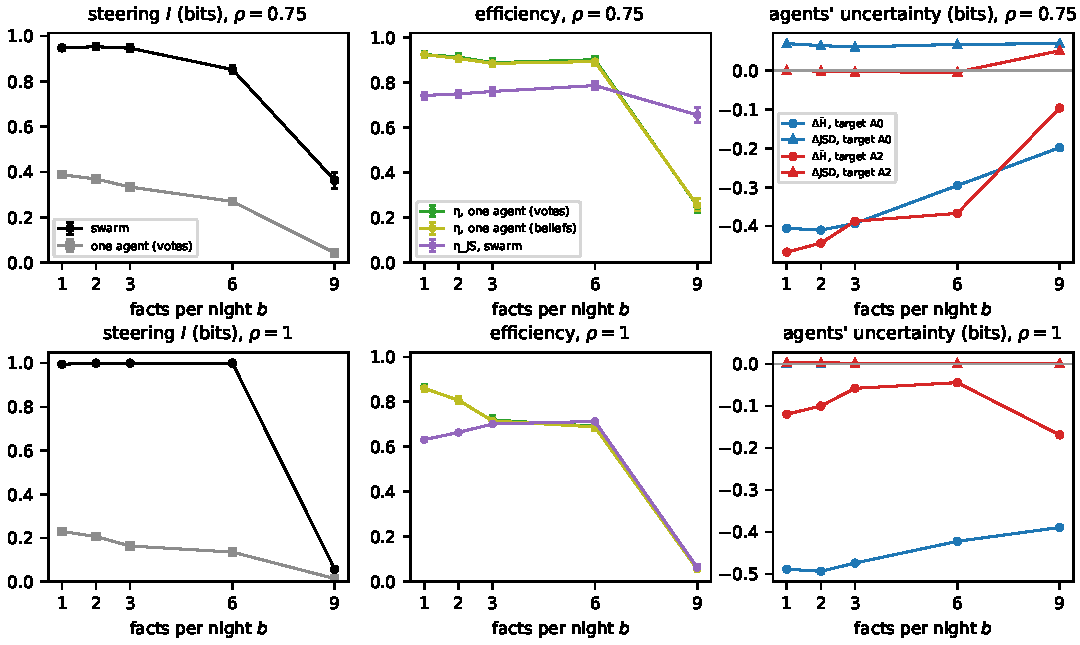
\includegraphics[width=0.72\linewidth]{figures/fig_eff_settings.pdf}
\caption{Readability $I$ (left), pair efficiency (middle) and the change in the agents' uncertainty
(right; circles $\Delta\bar H$, triangles $\Delta$JSD) at $t = 30$ against facts per night $b$ ($q_c = 12$). Bars: 95\% intervals.}
\label{fig:effsettings}
\end{figure}

\begin{itemize}\itemsep1pt
\item \textbf{$\eta$ collapses at $b = 9$} (0.25 at $\rho = 0.75$, 0.06 at $\rho = 1$) through a
  \emph{common push}: both controllers raise A0. Up to $b = 6$, at $\rho = 0.75$, the pair is balanced
  ($\eta \approx 0.9$).
\item The swarm-level readability saturates near 1 bit with full memory (every episode ends on its
  controller's side), so it measures distinguishability, not size; the one-agent readability is the
  informative measure there.
\end{itemize}

\subsection{Precision at 50, 100 and 300 paths}

\begin{table}[H]
\centering\small
\caption{Value from 1{,}000 paths per arm, and root-mean-square error of the estimate from 50, 100
or 300 paths (200 random subsets each), at $t = 30$, $b = 3$, $q_c = 12$, $\rho = 0.75$.}
\label{tab:effprec}
\begin{tabular}{lcccc}
\toprule
quantity & 1{,}000 paths & error, 50 & error, 100 & error, 300 \\
\midrule
steering $I$, swarm (3 bins) & 0.946 & 0.034 & 0.024 & 0.012 \\
steering $I$, one agent (votes) & 0.333 & 0.027 & 0.019 & 0.009 \\
efficiency $\eta$, one agent (votes) & 0.889 & 0.038 & 0.027 & 0.013 \\
efficiency $\eta_{JS}$, swarm & 0.761 & 0.038 & 0.025 & 0.013 \\
$\Delta\bar H$, target A0 & -0.393 & 0.036 & 0.026 & 0.012 \\
$\Delta\bar H$, target A2 & -0.387 & 0.034 & 0.025 & 0.012 \\
$\Delta$JSD, target A0 & 0.061 & 0.010 & 0.006 & 0.004 \\
$\Delta$JSD, target A2 & -0.003 & 0.009 & 0.006 & 0.003 \\
\bottomrule
\end{tabular}
\end{table}

\noindent Across all settings, at 100 paths: readability $\pm0.01$ (one agent) to $\pm0.03$ (swarm),
$\eta$ $\pm0.02$--$0.03$, $\Delta\bar H$ $\pm0.02$, $\Delta$JSD $\pm0.006$. Two settings that differ by
at least 0.02 are ordered correctly in 90--100\% of subsets.

%% ---------------------------------------------------------------------------------------------
\section{Success against facts posted}\label{sec:success}

The information measures above say how readable the command is, not whether the swarm ends up
deciding what the controller wants, nor at what cost. Here we measure both directly.

\begin{itemize}\itemsep1pt
\item \textbf{Collective decision} $Y_T$: plurality of the agents' last votes at time $T$; a tie
  between $k$ answers counts $1/k$. \textbf{Success}: $Y_T$ = the controller's target.
\item \textbf{Benefit} $\Delta_\pi = p_\pi - p_0$: change in the probability that the target wins,
  against the silent arm of the same episodes; $p_0$ is the silent probability.
\item \textbf{Cost} $C_\pi$: facts actually posted up to $T$, mean per run (not the allowed budget).
\item \textbf{Best-achievable curve} among the tested settings $\pi$ of one group ($\rho$, target):
  $\Delta^*(B) = \max\{\Delta_\pi : C_\pi \le B\}$, the largest gain reached spending at most $B$;
  read the other way, $C^*(\delta) = \min\{C_\pi : \Delta_\pi \ge \delta\}$, the least spending that
  reaches $\delta$. A setting below the curve is \emph{dominated}: another reached at least as much for less.
\item \textbf{Cost efficiency} $\eta_{\text{cost}} = C^*(\Delta_\pi)/C_\pi$: the share of the spending that
  was necessary (1: nothing cheaper reached as much). Not defined where $\Delta_\pi \le 0$ or its
  95\% interval includes 0.
\end{itemize}

\paragraph{How to read the curves.} Each dot is one setting, at (facts posted, gain). The
\textbf{solid line} is the best-achievable curve over the tested settings: it starts at $(0,0)$ (no
control) and steps up each time a setting reaches a higher gain than anything cheaper; dots on it have
$\eta_{\text{cost}} = 1$, dots below it are dominated, and $\eta_{\text{cost}}$ is how far to the left the
curve reaches the same gain. The \textbf{dashed line} is what becomes reachable if the controller
\emph{chooses its setting at random for each run}: using setting X (7 facts, $+0.32$) in half of the
runs and no control in the other half costs 3.5 facts and gains $+0.16$ \emph{on average}, so every
point on the straight segment between two settings (or between a setting and $(0,0)$) is reachable on
average; the dashed line is the outermost such segments (the concave hull through $(0,0)$). It lies above
the solid line where mixing beats every single setting. Its first segment from $(0,0)$ is arithmetic,
not an observation.

\begin{center}
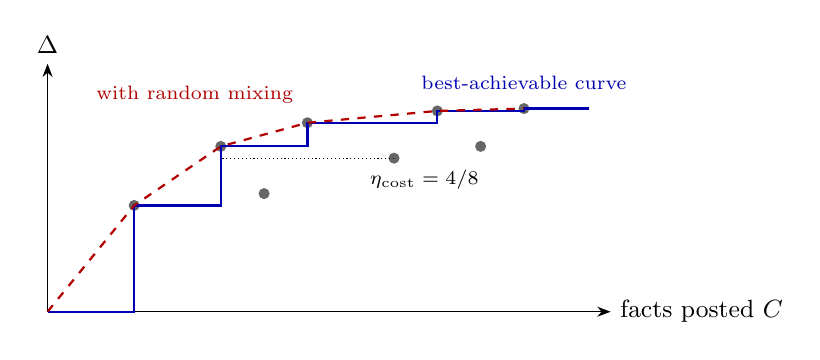
\begin{tikzpicture}[font=\small, x=0.55cm, y=3cm]
  \draw[-{Stealth}] (0,0) -- (13,0) node[right]{facts posted $C$};
  \draw[-{Stealth}] (0,0) -- (0,1.05) node[above]{$\Delta$};
  \foreach \c/\d in {2/0.45, 4/0.7, 6/0.8, 9/0.85, 11/0.86, 5/0.5, 8/0.65, 10/0.7}
     \fill[black!60] (\c,\d) circle (2pt);
  \draw[thick, blue!70!black] (0,0) -- (2,0) -- (2,0.45) -- (4,0.45) -- (4,0.7) -- (6,0.7) -- (6,0.8) -- (9,0.8) -- (9,0.85) -- (11,0.85) -- (11,0.86) -- (12.5,0.86);
  \draw[thick, dashed, red!70!black] (0,0) -- (2,0.45) -- (4,0.7) -- (6,0.8) -- (9,0.85) -- (11,0.86);
  \draw[densely dotted] (8,0.65) -- (4,0.65);
  \node[font=\scriptsize, align=left] at (8.7,0.56) {$\eta_{\text{cost}} = 4/8$};
  \node[font=\scriptsize, blue!70!black] at (11,0.97) {best-achievable curve};
  \node[font=\scriptsize, red!70!black] at (3.4,0.92) {with random mixing};
\end{tikzpicture}
\diagramcaption{Illustration. Each point is a setting. Solid: best-achievable curve; dashed: reachable
on average by random mixing per run. The setting at cost 8 reaches $\Delta = 0.65$, which a setting
costing 4 already reaches: $\eta_{\text{cost}} = 0.5$.}
\end{center}

\begin{figure}[H]
\centering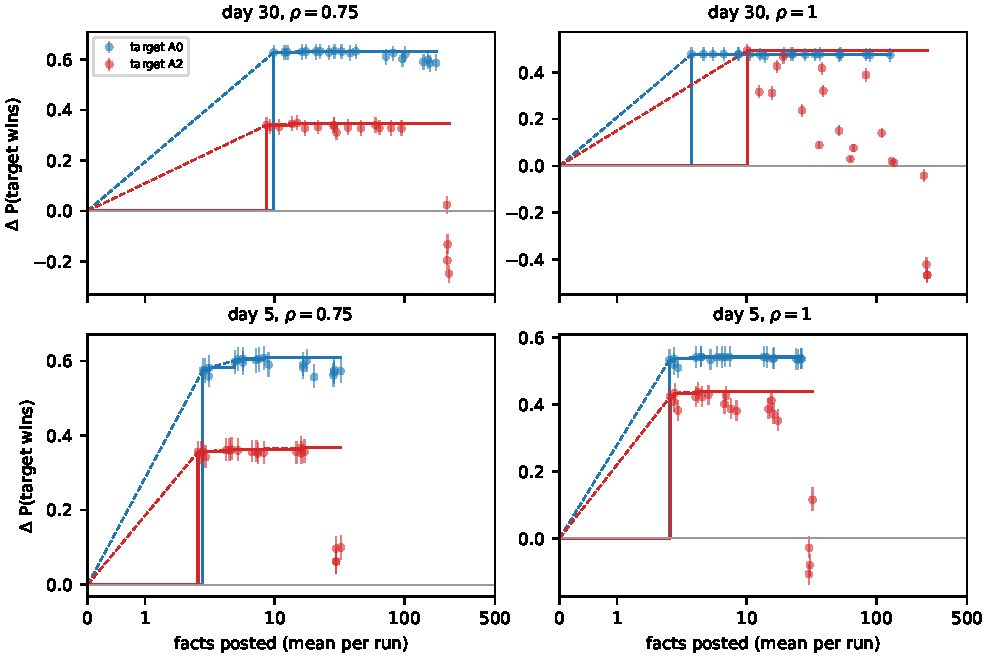
\includegraphics[width=0.84\linewidth]{figures/fig_success_facts.pdf}
\caption{Change in the probability that the controller's target wins against facts posted, on day
30 (top) and day 5 (bottom), $\rho = 0.75$ (left) and $1$ (right); every setting ($q_c \times b$,
$q = 6$, probability matching) with its 95\% interval; blue: target A0, red: target A2. Solid:
best-achievable curve; dashed: with random mixing per run. The x axis is linear from 0 to 1 and
logarithmic above, up to 500.}
\label{fig:success}
\end{figure}

\begin{itemize}\itemsep1pt
\item \textbf{On day 30 success saturates with very little control.} When agents forget, the cheapest
  setting ($q_c = 12$, $b = 1$) already reaches the full gain: $+0.63$ for target A0 with 9.8 facts,
  $+0.34$ for target A2 with 8.7 facts. Larger budgets reach the same gain or less with up to
  18 times more facts (median $\eta_{\text{cost}}$ 0.43 for target A0, 0.30 for A2; down to 0.06).
\item \textbf{Large budgets backfire in success too}: at $b = 9$ the false controller \emph{lowers} the
  chance that A2 wins (down to $-0.25$ at $\rho = 0.75$ and $-0.47$ at $\rho = 1$) after posting
  about 220--250 facts (Section~\ref{sec:strength}); no efficiency is defined there.
\item \textbf{With full memory only one setting is efficient} for each target ($q_c = 24$, $b = 1$:
  3.7 facts for $+0.48$, target A0; 10 facts for $+0.49$, target A2).
\item \textbf{By day 5 the swarm is already decided.} The cheapest settings (2.5--2.8 facts) reach
  nearly the full day-5 gain ($+0.57$ of $+0.61$ for target A0, $+0.36$ of $+0.37$ for A2, $\rho =
  0.75$): unlike Simulation 2 at $t = 5$, speed buys little. Here the swarm tips within about three
  days (Table~\ref{tab:pm}), so by day 5 the decision is mostly settled whatever the budget.
\item \textbf{Target A0 gains more than A2 mostly because of where the silent swarm starts}: without
  control A2 wins 63\% of runs and A0 36\% when agents forget. As a share of the room left,
  $\Delta/(1-p_0)$, the targets are closer (median 0.99 for A0, 0.90 for A2).
\item \textbf{Precision at 100 paths}: $\Delta$ $\pm0.04$; $\eta_{\text{cost}}$ $\pm0.02$--$0.035$. Where gains
  are flat, which setting is ``on the curve'' is decided by differences smaller than this.
\end{itemize}

%% ---------------------------------------------------------------------------------------------
\section{Specific to Simulation 1: the A2 drift under argmax voting}\label{sec:drift}

Simulation 2 has only probability-matching agents, so this section has no counterpart there.

\begin{figure}[H]
\centering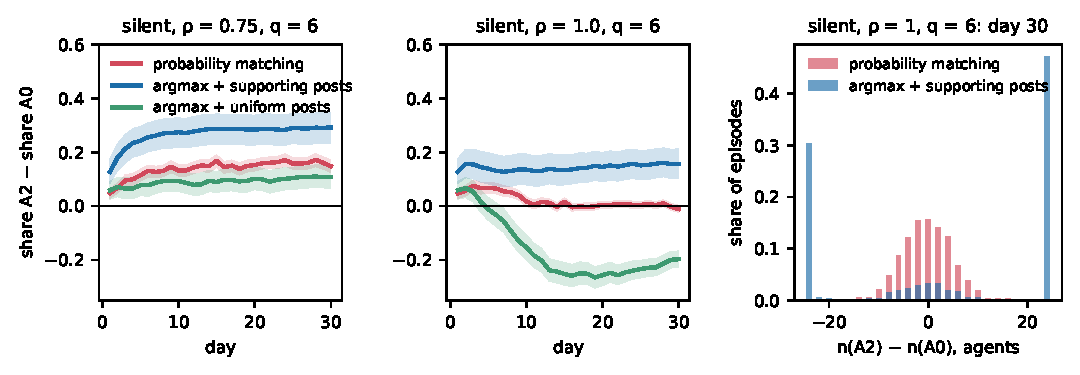
\includegraphics[width=0.98\linewidth]{figures/fig_drift.pdf}
\caption{Silent arm, $q = 6$. Left and middle: A2 $-$ A0 vote margin over the days.
Right: day-30 spread of the margin across episodes, in agents.}
\label{fig:drift}
\end{figure}

With argmax voting and vote-supporting posts (the \emph{base} rule), the silent swarm does
not stay undecided: \textbf{63--91\% of episodes end unanimous}, all 24 agents on A2
(43--67\%) or on A0 (15--41\%). The mean margin toward A2 (Figure~\ref{fig:drift}, blue)
is the difference between those two groups; the histogram shows the lock-in at
$\pm 24$. Under probability matching (red) the margin stays near zero: exactly 0 with full memory, and
a small lean of +0.07 to +0.15 toward A2 when agents forget. Three ingredients combine:

\begin{enumerate}\itemsep1pt
\item \textbf{Argmax turns any lead into a vote}, Eq.~(\ref{eq:argmax}).
\item \textbf{Agents post only facts supporting their vote}, so later readers mostly meet
  the majority's evidence, and with forgetting the minority's evidence dies out
  (day 30, $\rho = 0.75$: A2-side facts held by 53\% of agents, A0-side by 24\%).
\item \textbf{The swarm starts with more A2 voters.} Under argmax, an agent holding a fact
  that favours two allocations equally votes for each half the time. Its expected
  starting vote is
  \begin{equation}\label{eq:startvote}
  \mathbb{E}[n_k] = \sum_{j=1}^{24} \frac{\mathbb{1}\{k \in \arg\max P_j\}}{|\arg\max P_j|},
  \end{equation}
  which gives \textbf{7 / 6 / 11} for A0 / A1 / A2 (Table~\ref{tab:start}).
\end{enumerate}
Remove ingredient 1 (probability matching) or 2 (uniform posting: post any remembered
fact) and the lock-in collapses: no unanimous episode at all under probability matching,
9--22\% under uniform posting.

\begin{table}[H]
\centering\small
\caption{Why the start is 7 / 6 / 11. The setup balanced agents by \emph{fact group}
(8 per allocation), assigning a tied fact to the lower-numbered allocation; argmax votes
split ties.}
\label{tab:start}
\begin{tabular}{lccc}
\toprule
 & A0 & A1 & A2 \\
\midrule
agents per fact group (design bookkeeping) & 8 & 8 & 8 \\
\quad of which hold a fact tied A1/A2 (counted as A1) & -- & 6 & -- \\
\quad of which hold a fact tied A0/A1 (counted as A0) & 2 & -- & -- \\
expected starting votes, argmax, Eq.~(\ref{eq:startvote}) & \textbf{7} & \textbf{6} & \textbf{11} \\
expected starting votes, probability matching & 8.3 & 7.4 & 8.3 \\
\bottomrule
\end{tabular}
\end{table}

\paragraph{How to fix the start.} Balance the agents on \emph{expected votes},
Eq.~(\ref{eq:startvote}), instead of on fact groups. Under the current rules this is
impossible: none of the 10,438 coin-flip agent sets the builder can produce has equal
expected A0 and A2 votes. The reason is scarcity: only 3 eligible facts favour A1
alone, so any 5-fact A1 group must include A1/A2-tied facts. Dropping the
fact-group rule and requiring expected votes of exactly 8 / 8 / 8 directly works: a
random search found such agent sets (still a coin flip, all facts eligible), e.g.\ 12
facts each held by 2 agents. A full rebuild would also re-check the pool rules (no
shared facts, no joint proof). This changes the frozen setup, so it is a decision, not
yet applied. Probability matching needs no fix: its start is already balanced.

\paragraph{Caveats.} One world (task\_003), 24 agents, exact-Bayesian agents; means over
1,000 episodes per cell. Efficiencies are relative to the tested settings: nothing was tested below
about 2.5 facts (day 5) or 4 facts (day 30). Full analysis, code and tables:
\texttt{analysis/task003\_llm\_free/simulation\_1/analysis/} (reports Q0--Q6) and
\texttt{analysis/task003\_llm\_free/efficiency\_estimates/}.

\end{document}
